\subsection{Регистрация дисконтных карт}
\subsubsection{Описание изменений в процессе регистрации дисконтных карт	}
\begin{itemize}	
	\item Изменения внесенные в процесс регистрации новой дисконтной карты. Теперь запись нового элемента справочника (новой дисконтной карты) произойдет только если будет указан верный вид дисконтной карты. Тот, который указан в настройках программы.
		\sidenote[-2ex][]{Есть возможность в настройках изменить тип карты}.
	\begin{figure}[H]
		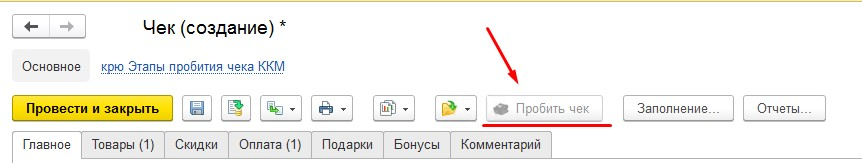
\includegraphics[width=0.8\textwidth]{30.jpg}
		\caption{Запрет записи.}
		\label{ris:30.jpg}
	\end{figure}

\end{itemize}